\section{Breitensuche}
\label{subsec:module.Suchalgorithmen.Breitensuche}
Die Breitensuche (engl. Breadth First Search (\gls{BFS})) war eine der Neuimplementierungen w�hrend der Bachelorarbeit. Wir verwenden diese Suche um die Umgebung einer Ameise oder eines H�gels nach Futter, Gegnern usw. zu scannen. Man k�nnte die \gls{BFS} auch f�r die Pfadsuche verwenden, dies w�re aber sehr ineffizient. Im Klassendiagramm ist zu sehen auf welchen drei Methoden die Breitensuche aufbaut.

Der Algorithmus f�r die Breitensuche ist in \cite{AIMA} beschrieben und wurde nach dieser Beschreibung implementiert.

\begin{figure}[H]
\centering
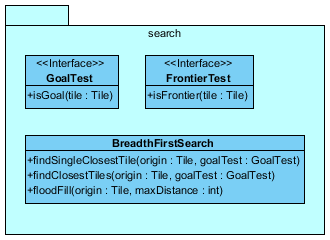
\includegraphics[width=0.6\textwidth]{91_bilder/BFS}
\caption{Breitensuche Klassendiagramm}
\label{fig:BFS}
\end{figure}

Die Breitensuche wurde generisch implementiert, so dass sie vielseitig einsetzbar ist. So k�nnen zum Beispiel mittels 'GoalTest' je nach Anwendungsfall die Tiles beschrieben werden die gesucht sind. Folgende Breitensuche findet die Ameise welche am n�chsten bei einem Food-Tile <r:20,c:16> ist. Die Suche wird initialisiert indem im Konstruktor die Spielkarte mitgegeben wird, welche durchforscht wird. Zus�tzlich gilt die Einschr�nkung das die Breitensuche nur 40 Tiles durchsuchen darf, was einem Radius von zirka 7 Zellen entspricht. Falls keine Ameise gefunden wird gibt der Algorithmus NULL zur�ck.

\lstset{language=Java, tabsize=4}
\begin{lstlisting}
AntsBreadthFirstSearch bfs = new AntsBreadthFirstSearch(Ants.getWorld());
Tile food = new Tile(20,16);
Tile antClosestToFood = bfs.findSingleClosestTile(food, 40, new GoalTest() {
      @Override
      public boolean isGoal(Tile tile) {
          return isAntOnTile(tile);
      }
  });
\end{lstlisting}

Es ist auch m�glich mehrere Tiles zur�ck zu bekommen. Dazu wird die Methode \texttt{findClosestTiles(...)} aufgerufen.\\
\\
Der gleiche Algorithmus kann aber auch alle passierbaren Tiles in einem gewissen Umkreis zur�ckgeben. Dies haben wir unter anderem beim Initialisieren der DefendHillMission verwendet. Wir berechnen beim Erstellen der Mission die passierbaren Zellen rund um den H�gel. Runde f�r Runde pr�fen wir diese Tiles auf gegnerische Ameisen um die entsprechenden Verteidigungsmassnahmen zu ergreifen. Der Parameter controlAreaRadius2 definiert den Radius des 'Radars' und kann je nach Profil unterschiedlich eingestellt werden.

Dieser Flood Fill Algorithmus ist praktisch identisch mit der Breitensuche. Eine Beschreibung von Flood Fill befindet sich in \cite{ARTIFICIALINTELLIGENCEFORGAMES}.

\lstset{language=Java, tabsize=4}
\begin{lstlisting}
public DefendHillMission(Tile myhill) {
    this.hill = myhill;
    BreadthFirstSearch bfs = new BreadthFirstSearch(Ants.getWorld());
    tilesAroundHill = bfs.floodFill(myhill, controlAreaRadius2);
}
\end{lstlisting}


Um die Aufrufe der Suche im Ants-Umfeld einfacher zu gestalten haben wir die Breitensuche f�r unseren Bot mit folgenden selbst-sprechenden Methoden erweitert.

\begin{figure}[H]
\centering
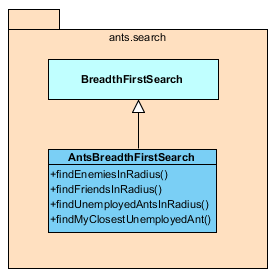
\includegraphics[width=0.5\textwidth]{91_bilder/BFSants}
\caption{Breitensuche Ants-spezifisch}
\label{fig:BFSants}
\end{figure}


\subsection{Barrier (Sperre)}
\label{subsec:module.Suchalgorithmen.Breitensuche.Barrier}

Eine Erweiterung der Breitensuche erm�glicht uns eine Sperre in der Umgebung eines Ortes zu finden. Diese Verwenden wir in der DefendHillMission zum Verteidigen des eigenen H�gels. Es kann nur eine Sperre (engl. Barrier) gefunden werden wenn das Gel�nde dazu passt. Die Abbildung \ref{fig:search.barrier} zeigt eine solche gefundene Sperre. Auf dieser H�he wird der H�gel verteidigt.

\begin{figure}[H]
\centering
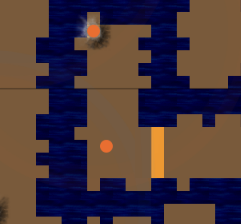
\includegraphics[width=0.5\textwidth]{91_bilder/barrier}
\caption{Auf der orangen Sperre werden die Ameisen zur Verteidigung des H�gel positioniert.}
\label{fig:search.barrier}
\end{figure}

Der Algorithmus ist in der Methode \texttt{getBarrier(...)} implementiert. Diese wird aufgerufen mit den Parametern \texttt{tileToProtect} (Ort der durch eine Sperre gesch�tzt werden soll), \texttt{viewRadiusSquared} (den Sichtradius der Einheiten), denn die Sperre soll weiter entfernt sein als der Sichtradius, damit die gegnerischen Einheiten nicht sehen was sich dahinter verbirgt. Der dritte Parameter \texttt{maximumBarrierSize} definiert, welche Breite die Sperre maximal haben darf.

\lstset{language=Java, tabsize=4}
\begin{lstlisting}
public Barrier getBarrier(final Tile tileToProtect, int viewRadiusSquared, int maximumBarrierSize) {

	//BFS for getting the amount of tiles in view radius around the location to defend.
	int amount = [...]
	Barrier smallestBarrier = null;
	List<Tile> tiles = get (amount + 30) tiles around the location to defend.
	
	// for loop start at the first tile not in view radius
	for(int i = amount;i<tiles.size(); i++){       
		Tile t = tiles.get(i);
		
		//vertical check
		if(!barrierVerticalInvalid.contains(t)){
			Barrier b = get vertical barrier on position of Tile t
			if(b is smaller than 5 Tiles && smaller than smallestBarrier){
				if(is barrier the only exit out of the location to defend){
						smallestBarrier = b;
				}else{
						 //add all tiles of the invaild barrier
						barrierVerticalInvalid.add(b.getTiles());
				}    					      		
			}else{
				 //add all tiles of the invaild barrier
				barrierVerticalInvalid.add(b.getTiles());
			}
		}
		
		//horizontal check
		if(!barrierHorizontalInvalid.contains(t)){
			Barrier b = get horiontal barrier on position of Tile t
			if(b is smaller than 5 Tiles && smaller than smallestBarrier){
				if(is barrier the only exit out of the location to defend){
						smallestBarrier = b;
				}else{
						 //add all tiles of the invalid barrier
						barrierHorizontalInvalid.add(b.getTiles());
				}    					      		
			}else{
				//add all tiles of the invalid barrier
				barrierHorizontalInvalid.add(b.getTiles());
			}
		}	
	}
}
\end{lstlisting}

Dank dem Abspeichern der ung�ltigen Tiles aller zu breiten Sperren in die Listen \texttt{barrierHorizontalInvalid} und \texttt{barrierVerticalInvalid} konnte der Algorithmus markant schneller gemacht werden. F�r diese Tiles muss nicht nochmals eine Sperre berechnet werden. Auch die if-Abfrage \texttt{barrier is the only exit out of the location to defend} muss nicht mehr oft aufgerufen werden, den hinter dieser Abfrage steht n�mlich wiederum ein Test mit der Breitensuche. Dieser zus�tzliche Test mit der Breitensuche ist viel teurer als das Zwischenspeichern der Tiles aus welchen keine g�ltige Sperre gemacht werden konnte.\\
\\
Im Nachhinein hat sich ergeben, dass nicht unbedingt die schmalste Sperre die Beste w�re, sondern jede bei welche der Gegner, gel�ndebedingt, weniger Einheiten aufstellen kann. So w�re in Abbildung \ref{fig:search.barrier} eine Sperre zwei Zellen �stlicher besser, den der Gegner k�nnte beim Angriff nur mit vier Einheiten vorr�cken, die Verteidigung w�re aber mit sechs Einheiten auf einer Linie deutlich st�rker. Die Zeit hat aber hier leider nicht gereicht, den Algorithmus weiter zu verfeinern.